% !TEX root = main.tex

% \begin{table}[t]
% 	\caption {Summary of datasets}
% 	\label{tab:datasets}
% 	\centering
% 	\begin{tabular}{llll}
% 		\toprule
% 		  & GoodNews  & GoodNews+ &   NYTimes800k \\
% 		\midrule
%       No. of articles & 241 808 & 241 808 & 445 828 \\
%       No. of images   & 462 642 & 440 112 & 794 085 \\
%       Article length & 451 & 963 & 974 \\
%       Caption length & 18 & 18 & 18 \\
%       Start month & Jan 10 & Jan 10 & Mar 05\\
%       End month & Jul 18 & Jul 18 & Sep 19 \\
% 		\bottomrule
% 	\end{tabular}
% \end{table}


\section{News Image Captioning Datasets}
\label{sec:dataset}
We describe two datasets that contain news articles, images, and captions. The
first dataset, GoodNews, was recently proposed in Biten
\etal~\cite{Biten2019GoodNews}, while the
second dataset, NYTimes800k, is our contribution.


\noindent{\bf GoodNews:}
The GoodNews dataset was previously the largest dataset for news image
captioning~\cite{Biten2019GoodNews}. Each example in the dataset is a triplet
containing an article, an image, and a caption. Since only the article text,
captions, and image URLs are publicly released, the images need to be
downloaded from the original source. Out of the 466K image URLs provided by
\cite{Biten2019GoodNews}, we were able to download 463K images, or 99.2\% of
the original dataset---the remaining are broken links.

We use this 99.2\% sample of GoodNews and the train-validation-test split
provided by~\cite{Biten2019GoodNews}. There are 421K training, 18K validation,
and 23K test captions. Note that this split was performed at the level of
captions, so it is possible for a training and test caption to share the same
article text (since articles have multiple images).

We observe several issues with GoodNews that may limit a system's
ability to generate high-quality captions. Many of the articles in GoodNews are
partially extracted because the generic article extraction library
failed to recognize some of the HTML tags specific to The New York Times.
Importantly, the missing text often included the first few paragraphs which
frequently contain important information for captioning images. In addition
GoodNews contains some non-English articles and captioned images from the
recommendation sidebar which are not related to the main article.


\begin{table}[t]
	\caption {Summary of news captioning datasets}
	\label{tab:datasets}
	\centering
	\begin{tabularx}{\linewidth}{lXX}
		\toprule
		  & GoodNews  &   NYTimes800k \\
		\midrule
      Number of articles & 257 033 & 444 914 \\
      Number of images   & 462 642 & 792 971 \\
      Average article length & 451 & 974 \\
      Average caption length & 18 & 18 \\
      Collection start month & Jan 10 & Mar 05\\
      Collection end month & Mar 18 & Aug 19 \\
      \midrule
      \multicolumn{2}{l}{\% of caption words that are}  \\
      \quad -- nouns & 16\% & 16\% \\
      \quad -- pronouns & 1\% & 1\% \\
      \quad -- proper nouns & 23\% & 22\% \\
      \quad -- verbs & 9\% & 9\%  \\
      \quad -- adjectives & 4\% & 4\% \\
      \quad -- named entities & 27\% & 26\% \\
      \quad\quad -- people's names & 9\% & 9\% \\
      \midrule
      \% of captions with \\
      \quad -- named entities & 97\% & 96\% \\
      \quad\quad -- people's names & 68\% & 68\% \\
		\bottomrule
	\end{tabularx}
\end{table}


\noindent{\bf NYTimes800k:}
The aforementioned issues motivated us to construct NYTimes800k, a 70\% larger
and more complete dataset of New York Times articles, images, and captions. We
used The New York Times public
API\footnote{\href{https://developer.nytimes.com/apis}{https://developer.nytimes.com/apis}}
for the data collection and developed a custom parser to resolve the missing
text issue in GoodNews. The average article in NYTimes800k is 963 words long,
whereas the average article in GoodNews is 451 words long. Our parser also
ensures that NYTimes800k only contains English articles and images that are
part of the main article. Finally, we also collect information about where an
image is located in the corresponding article. Most news articles have one
image at the top that relates to the key topic. However 39\% of the articles
have at least one more image somewhere in the middle of text. The image
placement and the text surrounding the image is important information for
captioning as we will show in our evaluations. Table~\ref{tab:datasets}
presents a comparison between GoodNews and NYTimes800k.

\begin{figure}[t]
   \begin{center}
   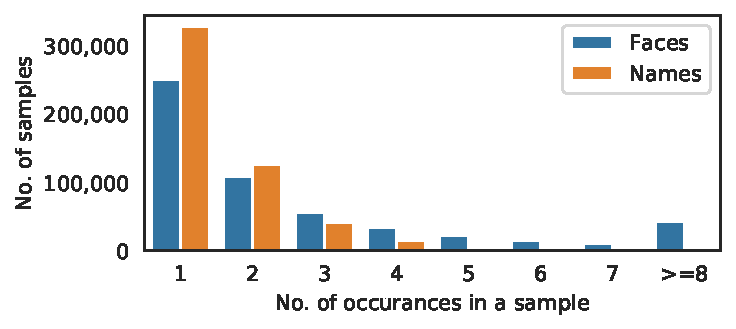
\includegraphics[width=0.99\linewidth]{figures/figure_3_faces.pdf}
   \end{center}
  \capmoveup
      \caption{Co-occurrence of faces and people's names in NYTimes800k
               training data. The blue bars count how many images containing a
               certain number of faces. The orange bars count how many captions
               containing a certain number of people's names.}
   \vspace{-3.5mm}
   \label{fig:faces}
\end{figure}





Entities play an important role in NYTimes800k, with 97\% of captions
containing at least one named entity. The most popular entity type are names of
people, comprising a third of all named entities (see the supplementary
material for a detailed breakdown of entity types). Furthermore, 71\% of
training images contain at least one face and 68\% of training captions mention
at least one person's name. Figure \ref{fig:faces} provides a further breakdown
of the co-occurrence of faces and people's names. One important observation is
that 99\% of captions contain at most four names.


We split the training, validation, and test sets according to time, as shown in
Table~\ref{tab:splits}. Compared to the random split used in GoodNews,
splitting by time allows us to study the model performance on novel news events
and new names, which might be important in a deployment scenario. Out of the
100K proper nouns in our test captions, 4\% never appear in any training
captions.
